% 请确保文件编码为utf-8,使用XeLaTex进行编译,或者通过overleaf进行编译

\documentclass[answers]{exam}  % 使用此行带有作答模块
% \documentclass{exam} % 使用此行只显示题目

\usepackage{xeCJK}
\usepackage{zhnumber}
\usepackage{graphicx}
\usepackage{hyperref}
\usepackage{amsmath}
\usepackage{amssymb}
\usepackage{mathtools}
\usepackage{booktabs}
\usepackage{enumerate}
\usepackage{enumitem} % 控制列表样式
\usepackage{listings} 

\title{2025模式识别 \\ 作业二}
\date{2025.3.25}
\pagestyle{headandfoot}
\author{人工智能学院 221300079 王俊童}
\firstpageheadrule
\firstpageheader{南京大学}{2025模式识别}{作业二}
\runningheader{南京大学}
{2025模式识别}
{作业二}
\runningheadrule
\firstpagefooter{}{第\thepage\ 页(共\numpages 页)}{}
\runningfooter{}{第\thepage\ 页(共\numpages 页)}{}

% no box for solutions
% \unframedsolutions
\def \x \mathbf{x}


\setlength\linefillheight{.5in}

% \renewcommand{\solutiontitle}{\noindent\textbf{答:}}
\renewcommand{\solutiontitle}{\noindent\textbf{解:}\par\noindent}

\renewcommand{\thequestion}{\zhnum{question}}
\renewcommand{\questionlabel}{\thequestion .}
\renewcommand{\thepartno}{\arabic{partno}}
\renewcommand{\partlabel}{\thepartno .}

\def\dist{{\mathrm{dist}}}
\def\x{{\boldsymbol{x}}}
\def\w{{\boldsymbol{w}}}


\begin{document}
% \normalsize
\maketitle
221300079 王俊童,人工智能学院
\section{问题一}
\begin{enumerate}[label=\alph*.] 
    \item 对于这个形式化问题,根据题目的描述如下:$\gamma_{ij}$表示第j个样本(共M
    个被分到了第i类别(共K类)。而$\mu_i$代表这个类别的均值。那很显然的一个事情是,我们的
    分类标准应该是类内是要尽量小的,意思是离均值点的距离应当近。因此我们的目标是,对于每一个类别
    都要做到这一点,那对应样本应该被分进正确的类别以达到最小,问题形式化如下:
    \begin{equation*}
        \mathcal{L} =\sum_{i=1}^{K}\sum_{j=1}^{M}\gamma_{ij}\|x_j-\mu_i\|
    \end{equation*}
    那么优化函数就可以写为题目说的那个样子:
    \begin{equation}
        \label{eq:1}
        \mathop{\arg\min}_{\gamma_{ij},\mu_i} \sum_{i=1}^{K}\sum_{j=1}^{M}\gamma_{ij}\|x_j-\mu_i\|
    \end{equation}
    QED,Eqn.~\ref{eq:1}

    \item 根据题目描述,第一步应该是$\mu_i$被固定,那么优化问题就变成了对于M个样本,我们要做到优化对于每个样本来说:
    \begin{equation*}
        \mathcal{L}_j = \sum_{i=1}^{K} \gamma_{ij}\|x_j - \mu_i\|^2
    \end{equation*}
    要做到上述的j个(共M个式子)最小,意思是属于某一个类别。那么对于这个东西,相当于求一个
    \begin{equation*}
        \mathop{\arg\min}_{i} \|x_j - \mu_i\|^2
    \end{equation*}
    只要找到了最小的,其他的标识变量都是0了。所以$\gamma_{ij}$可以重写为:
    \begin{equation}
        \gamma_{ij} = 
        \begin{cases}
            1, if\ dist = min_i \|x_j - \mu_i\|^2\\
            0, otherwise.
        \end{cases}
    \end{equation}
    对于第二步骤,其实是固定了类别之后,需要重新找一个分类的最小均值。此时问题变为:
    \begin{equation*}
        \label{eq:2}
        \mathcal{L}_i = \sum_{j=1}^{M}  \gamma_{ij}\|x_j - \mu_i\|^2
    \end{equation*}
    可以求导:
    \begin{equation*}
        \frac{\partial \mathcal{L}}{\partial \mu_i} = 0
    \end{equation*}
    可以解得:
    \begin{equation}
        \label{eq:3}
        \mu_i = \frac{\sum_{j=1}^{M}\gamma_{ij}x_j}{\sum_{j=1}^{M}\gamma_{ij}}
    \end{equation}
    所以这个题目的更新规则如Eqn.~\ref{eq:2},Eqn.~\ref{eq:3}所示。
    \item 证明敛散性,相当于证明,新得到的$\mathcal{L}' - \mathcal{L}$跟0的关系:\\
    对于步骤1,样本找到了一个新的类别,意思是找到了一个更小的均值点和他的距离,那么问题可以写为:
    \begin{equation*}
        \mathcal{L}' - \mathcal{L} = \sum_{i=1}^{K}\sum_{j=1}^{M}(\gamma_{ij}' - \gamma_{ij})\|x_j-\mu_i'\|^2
    \end{equation*}
    \begin{equation*}
        \mathcal{L}' - \mathcal{L} = \sum_{i=1}^{K}\sum_{j=1}^{M}(\|x_j-\mu_i'\|^2 - \|x_j-\mu_i\|^2)\leq 0
    \end{equation*}
    显然,根据刚才的证明,他会更小,所以一定成立。\\
    对于步骤2,只针对每一个类别来说,切换新的均值点,不增加计算成本,那么考虑一个类就行了:
    \begin{equation*}
        \mathcal{L}' - \mathcal{L} \sim \sum_{j=1}^{M}(\|x_j-\mu_i'\|^2 - \|x_j-\mu_i\|^2)
    \end{equation*}
    \begin{equation*}
        \mathcal{L}' - \mathcal{L} \sim \sum_{j=1}^{M}(\mu_i - \mu_i')^\top(2x_j - \mu_i - \mu_i')
    \end{equation*}
    将Eqn.~\ref{eq:3}带入可以化简得到:
    \begin{equation*}
        \mathcal{L}' - \mathcal{L} \sim -(\mu_i - \mu_i')^\top(\mu_i - \mu_i')\leq 0
    \end{equation*}
    那么,根据证明,确实收敛。
\end{enumerate}

\section{问题二}
\begin{enumerate}[label=\alph*.] 
    \item 把题目说的形式带进去可以了:
    \begin{equation*}
        \sum_{i=1}^{n} \epsilon_i^2 = \sum_{i=1}^{n} (y_i - \x_i^\top \mathbf{\beta})
    \end{equation*}
    \begin{equation*}
        \mathop{\arg\min}_{\mathbf{\beta}} \sum_{i=1}^{n} (y_i - \x_i^\top \mathbf{\beta})
    \end{equation*}
    \item 可以写成矩阵形式的优化问题:
    \begin{equation*}
        \mathop{\arg\min}_{\mathbf{\beta}} (\mathbf{y} - \mathbf{X} \mathbf{\beta})^\top (\mathbf{y} - \mathbf{X} \mathbf{\beta})
    \end{equation*}
    矩阵形式的优化问题就是这样。
    \item 可逆的话,那么用求导等于0就好了:
    \begin{equation*}
        \frac{\partial \mathcal{L}}{\partial \beta} = 2\mathbf{X}^\top (\mathbf{X}\beta - \mathbf{y}) = 0
    \end{equation*}
    \begin{equation*}
        \beta^* = (\mathbf{X}^\top\mathbf{X})^{-1} \mathbf{X}^\top \mathbf{y}
    \end{equation*}
    \item 因为维度d比n大,第二问说X是n*d的,那么$rank(\mathbf{X})\leq n<d$可以得到,那么$rank(\mathbf{X}^\top \mathbf{X})\leq n<d$可以得到。但是,
    $\mathbf{X}^\top\mathbf{X}$这个东西是d*d的,所以一定不满秩。那就不可逆了
    \item 在正则化项加入了之后,这个东西一般不可逆的,就可以求解了。而且一般模型都没有闭式解,这种
    情况下引入正则化项既降低了复杂度,也同时使得式子可以求解,这样就有闭式解了,一般为复杂度最低的,
    感觉也算是一种归纳偏好吧。
    \item 引入正则化之后的优化目标如下:
    \begin{equation*}
        \mathop{\arg\min}_{\mathbf{\beta}} (\mathbf{y} - \mathbf{X} \mathbf{\beta})^\top (\mathbf{y} - \mathbf{X} \mathbf{\beta}) + \lambda \mathbf{\beta}^\top \mathbf{\beta}
    \end{equation*}
    求导化简:
    \begin{equation*}
        \frac{\partial \mathcal{L}}{\partial \beta} = 2\mathbf{X}^\top (\mathbf{X}\beta - \mathbf{y}) + 2\lambda \mathbf{\beta}= 0
    \end{equation*}
    \begin{equation*}
        \beta^* = (\mathbf{X}^\top\mathbf{X} + \lambda \mathbf{I})^{-1} \mathbf{X}^\top \mathbf{y}
    \end{equation*}
    \item 上面说了,如果不可逆的时候,这样就解决不了了,因为没有唯一的闭式解了。但是这个东西加入之后,那个$\lambda\mathbf{I}$可以
    让基本所有情况都可以解。这个时候就可以选择了。
    \item $\lambda=0$,就变成之前的普通线性回归,$\lambda=\infty$,这个只能解后面的$\beta^\top\beta = 0$,答案就是0.
    \item 我觉得不行,假如我们可以找到最优解$\lambda^*, \beta^*$,那么原来的运算可以写作:
    \begin{equation*}
        (\mathbf{y} - \mathbf{X} \mathbf{\beta^*})^\top (\mathbf{y} - \mathbf{X} \mathbf{\beta^*}) + \lambda^* \mathbf{\beta^*}^\top \mathbf{\beta^*}
    \end{equation*}
    但是你会发现一个非常严肃的问题,当没有正则化的时候,一定存在:
    \begin{equation*}
        (\mathbf{y} - \mathbf{X} \mathbf{\beta^*})^\top (\mathbf{y} - \mathbf{X} \mathbf{\beta^*}) < (\mathbf{y} - \mathbf{X} \mathbf{\beta^*})^\top (\mathbf{y} - \mathbf{X} \mathbf{\beta^*}) + \lambda^* \mathbf{\beta^*}^\top \mathbf{\beta^*}
    \end{equation*}
    那不是,我令为0不就行了,所以没啥用。
\end{enumerate}


\section{问题三}
\begin{enumerate}[label=\alph*.] 
    \item 表格如下:
    \begin{table}[h]
        \centering
        \caption{Performance Metrics Table}
        \begin{tabular}{c|c|c|c|c|c|c}
            \hline
            下标 & 类别标记 & 得分 & 查准率 & 查全率 & AUC-PR & AP \\
            \hline
            0  & - & -   & 1.0000 & 0.0000 & -      & -      \\
            1  & 1 & 1.0 & 1.0000 & 0.2000 & 0.2000 & 0.2000 \\
            2  & 2 & 0.9 & 0.5000 & 0.2000 & 0.0000 & 0.0000 \\
            3  & 1 & 0.8 & 0.6667 & 0.4000 & 0.1167 & 0.1333 \\
            4  & 1 & 0.7 & 0.7500 & 0.6000 & 0.1417 & 0.1500 \\
            5  & 2 & 0.6 & 0.6000 & 0.6000 & 0.0000 & 0.0000 \\
            6  & 1 & 0.5 & 0.6667 & 0.8000 & 0.1267 & 0.1333 \\
            7  & 2 & 0.4 & 0.5714 & 0.8000 & 0.0000 & 0.0000 \\
            8  & 2 & 0.3 & 0.5000 & 0.8000 & 0.0000 & 0.0000 \\
            9  & 1 & 0.2 & 0.5556 & 1.0000 & 0.1056 & 0.1111 \\
            10 & 2 & 0.1 & 0.5000 & 1.0000 & 0.0000 & 0.0000 \\
            -  & - & -   & -      & -      & 0.6907 & 0.7277 \\
            \hline
        \end{tabular}
    \end{table}
    \item 由于AP的算法为
    \begin{equation*}
        AP = \sum_{i=1}^{n} (r_i - r_{i-1})*p_i
    \end{equation*}
    而AUC-PR为:
    \begin{equation*}
        AUC-PR = \sum_{i=1}^{n} (r_i - r_{i-1})*\frac{p_i+p_{i-1}}{2}
    \end{equation*}
    做个减法:
    \begin{equation*}
        AP -  AUC-PR = \sum_{i=1}^{n} (r_i - r_{i-1})*\frac{p_i - p_{i-1}}{2}
    \end{equation*}
    一般情况下$p_i \geq p_{i-1}$所以确实AP会比AUC大一些。
    \item 我们通过计算可以得到新的AUC为0.6794,新的AP为0.7167.其实就是跟先进入正样本还是负样本的顺序有区别罢了。
    \item 计算得到:AUC-PR: 0.6906,
    AP: 0.7278.说明我们算对了。
    图像如下:
    \begin{figure}[ht]
        \centering
        \label{auc}
        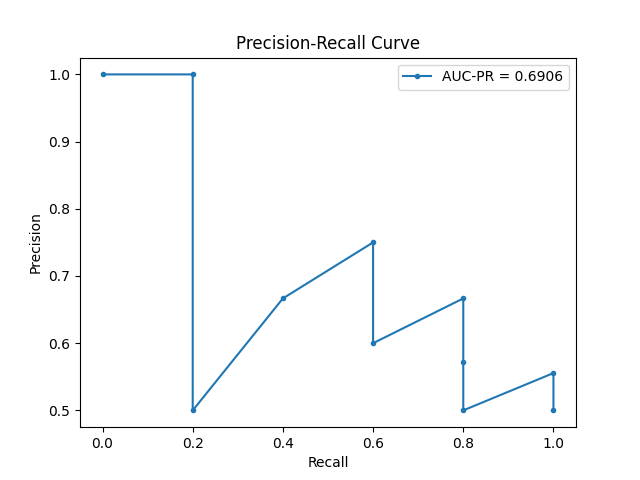
\includegraphics[width=0.8\textwidth]{pr.png} 
        \caption{auc}  
    \end{figure}
    代码如下:
    \begin{lstlisting}[language=Python, caption=Python代码示例, label=code:example, basicstyle=\ttfamily]
        import numpy as np
        import matplotlib.pyplot as plt
        from sklearn.metrics import precision_recall_curve, auc, average_precision_score

        data = [
            (0, 1, 1.0),
            (1, 2, 0.9),
            (2, 1, 0.8),
            (3, 1, 0.7),
            (4, 2, 0.6),
            (5, 1, 0.5),
            (6, 2, 0.4),
            (7, 2, 0.3),
            (8, 1, 0.2),
            (9, 2, 0.1)
        ]

        true_labels = np.array([label for _, label, _ in data])
        scores = np.array([score for _, _, score in data])

        binary_labels = (true_labels == 1).astype(int)
        precision, recall, _ = precision_recall_curve(binary_labels, scores)
        auc_pr = auc(recall, precision)
        ap = average_precision_score(binary_labels, scores)

        print(f"AUC-PR: {auc_pr:.4f}")
        print(f"AP: {ap:.4f}")

        plt.figure()
        plt.plot(recall, precision, marker='.', label=f'AUC-PR = {auc_pr:.4f}')
        plt.xlabel('Recall')
        plt.ylabel('Precision')
        plt.title('Precision-Recall Curve')
        plt.legend()
        plt.savefig('pr.png')
        plt.show()
    \end{lstlisting}
\end{enumerate}

\section{问题四}
\begin{enumerate}[label=\alph*.] 
    \item 对于这个问题,题目其实想验证一个问题,减去均值和不减去均值会对PCA造成什么影响。
    实际上,减去均值之后是对的,这样pca才能找到真正的变化方向。但是如果不减去均值,题目很有可能
    把第一主成分当作均值方向。我们可以看一下实验数据的表现。
    \begin{lstlisting}[language=matlab]
        Scale: 1.0000, corr1: -1.0000, corr2: 0.0373
        Scale: 0.5000, corr1: -1.0000, corr2: -0.3636
        Scale: 0.1000, corr1: 0.9982, corr2: 0.2976
        Scale: 0.0500, corr1: 0.9924, corr2: 0.1879
        Scale: 0.0100, corr1: 0.2269, corr2: 0.9921
        Scale: 0.0050, corr1: 0.1261, corr2: 0.9987
        Scale: 0.0010, corr1: 0.2926, corr2: 0.9999
        Scale: 0.0001, corr1: 0.0672, corr2: 1.0000
    \end{lstlisting}
    我们可以看到,scale很大的时候,未中心化 PCA 会使得第一主成分主要指向均值方向,这种影响最为明显。

    中心化后 PCA 的主成分 $new\_e1$ 更能反映数据的真实变异方向,而不是均值的影响。可以看到这个在scale越小的时候,越接近1.
    可以看出正确的第一主成分 $new\_e1$ 主要由数据的协方差决定,而不是均值,因此当 scale 变小时,它的方向稳定。

    通过这个题可以看出来,必须减去均值(中心化),在scale小的时候影响都不大的,这才是对的。不减均值那个完全就会
    导致整个方向错乱,甚至在scale大的时候,完全的被指向了与avg相反的方向,这是错误的。
    \begin{lstlisting}[language=matlab]
        rand('seed', 0);
        scales = [1, 0.5, 0.1, 0.05, 0.01, 0.005, 0.001, 0.0001];
        avg = [1 2 3 4 5 6 7 8 9 10];
        
        for scale = scales
            % 生成数据
            data = randn(5000, 10) + repmat(avg * scale, 5000, 1);
            
            % 计算均值并归一化
            m = mean(data);
            m1 = m / norm(m);
            
            % PCA without centering
            [~, S, V] = svd(data);
            S = diag(S);
            e1 = V(:,1);
            
            % PCA with centering
            newdata = data - repmat(m, 5000, 1);
            [U, S, V] = svd(newdata);
            S = diag(S);
            new_e1 = V(:,1);
            
            % 计算相关性
            avg_scaled = avg - mean(avg);
            avg_scaled = avg_scaled / norm(avg_scaled);
            
            e1 = e1 - mean(e1);
            e1 = e1 / norm(e1);
            
            new_e1 = new_e1 - mean(new_e1);
            new_e1 = new_e1 / norm(new_e1);
            
            corr1 = avg_scaled * e1;
            corr2 = e1' * new_e1;
            
            % 输出结果
            fprintf('Scale: %.4f, corr1: %.4f, corr2: %.4f\n', scale, corr1, corr2);
        end
    \end{lstlisting}
    当然,这个题还喊我们看正确的特征向量
    \begin{lstlisting}[language=matlab]
        Scale: 1.0000, corr1: -1.0000, corr2: -0.6733
        new_e1 (first 5 values): -0.3525 -0.2847 -0.4691 0.3433 -0.2291
        Scale: 0.5000, corr1: 1.0000, corr2: 0.1689
        new_e1 (first 5 values): -0.1231 -0.3047 0.2140 0.1848 0.0328
        Scale: 0.1000, corr1: 0.9988, corr2: -0.5822
        new_e1 (first 5 values): 0.4918 0.1268 0.2494 -0.0886 0.3937
        Scale: 0.0500, corr1: -0.9964, corr2: -0.4006
        new_e1 (first 5 values): -0.2049 -0.4067 -0.0147 0.4926 -0.0330
        Scale: 0.0100, corr1: 0.8100, corr2: 0.1957
        new_e1 (first 5 values): -0.0573 -0.1757 -0.4358 -0.1678 0.7425
        Scale: 0.0050, corr1: 0.2241, corr2: 0.9998
        new_e1 (first 5 values): -0.5281 0.4544 -0.1225 -0.3347 0.2780
        Scale: 0.0010, corr1: 0.1857, corr2: 1.0000
        new_e1 (first 5 values): 0.0536 0.0390 -0.4744 0.1108 0.0601
        Scale: 0.0001, corr1: 0.4436, corr2: 1.0000
        new_e1 (first 5 values): -0.0259 -0.2168 -0.7334 0.0134 0.4399
    \end{lstlisting}
    可以看出:当 scale 较大时(如 1.0 或 0.5),$new\_e1$ 的值有较大波动。例如,在 scale = 1.0 时,$new\_e1$ 的前五个值为:-0.3525 -0.2847 -0.4691 0.3433 -0.2291。这表明均值对数据影响较大,导致主成分的方向变化较大。
    当 scale 较小时(如 0.0010 或 0.0001),$new\_e1$ 趋于稳定。例如,在 scale = 0.0010 时,$new\_e1$ 的前五个值为:0.0536 0.0390 -0.4744 0.1108 0.0601,这表明数据的协方差结构主导了特征向量,主成分变得更稳定
\end{enumerate}

\section{问题五}
\begin{enumerate}[label=\alph*.] 
    \item 左乘一个G矩阵之后,对于x的改变就是$i,j$两个。可以得到基本为:
    \begin{equation*}
        y = 
        \begin{cases}
            cx_i - sx_j, if\ y_i\\
            sx_i + cx_j, if\ y_j\\
            y_k, k\neq i, k \neq j
        \end{cases}
    \end{equation*}
    \item 第j行的表达式为:$sx_i + cx_j = 0$, 所以有:$sx_i = -cx_j$
    \begin{equation*}
        \theta = \arctan(-\frac{x_j}{x_i})
    \end{equation*}
    这个时候就满足等于0了。等价的说,可以有这个式子:
    \begin{equation}
        \label{eq:4}
        c=\frac{x_i}{r},s=\frac{-x_j}{r},\ r=\sqrt{x_i^2+ x_j^2}
    \end{equation}
    \item 如果不用三角函数,就用上面的Eqn.~\ref{eq:4}.那么问题就化简为一个先计算r,然后
    \begin{itemize}
        \item if $r\neq 0$, 用Eqn.~\ref{eq:4}
        \item if $r=0$, c=1,s=0.既可
    \end{itemize}
    \item 会对A矩阵的第i行和第j行做改变,比如对于第i行的第一个元素,原来是$A_{i1}$,现在变成了$cA_{i1}-sA_{j1}$
    对于第j行也一样,只不过变成了$sA_{i1}+cA_{j1}$,其余的列在i,j行的变化也一样。总结就是
    \begin{equation*}
        A'_i=cA_i - sA_j, A'_j = sA_i +cA_j
    \end{equation*}
    假如我们要让其中的一个$A_{jk}$为0.那么则有$sA_{ik} + cA_{jk} = 0$,$\tan\theta = -\frac{A_{jk}}{A_{ik}}$
    那么则有:
    \begin{equation}
        \label{eq:5}
        c = \frac{A_{ik}}{\sqrt{A_{ik}^2 + A_{jk}^2}},s = -\frac{A_{jk}}{\sqrt{A_{ik}^2 + A_{jk}^2}}
    \end{equation}
    这样就为0了。

    复杂度这一块的话,如果只是单次Givens旋转,只修改2行,复杂度是O(n).
    \item  我们可以发现,对于QR分解,这个东西本质就是把一个矩阵变成一个Q,$Q^\top Q = I$,然后这个R还是个上三角。
    不难发现我们的Givens矩阵有一个很好的性质,对于任意的一个givens矩阵G来说,存在:
    \begin{equation*}
        G^\top G = I
    \end{equation*}
    也就是说,这个givens矩阵本身充当的就是帮助Q进行变换的角色。那么问题就简单了,不停的利用givens矩阵去小曲下三角的元素即可。
    
    那我们的思路就是,对于一个矩阵A来说,从左往右,从上往下去消去下三角部分的值,选
    $A_{ij},i>j$,构造givens让$A_{ij}=0$.我们可以选对角线元素,有Eqn.~\ref{eq:5}即可。重复这个过程,每次更新Q
    Q = QG即可。
    最后这个东西就是这么做的。

\end{enumerate}

\section{问题六}
\begin{enumerate}[label=\alph*.] 
    \item 根据谱范数和奇异值之间的定义可以得到$\|\mathbf{A}\|_2 = \sup_{\|\mathbf{x}\|_2 = 1} \|\mathbf{A}x\|_2 = \sigma_1$即最大的奇异值。
    所以可以得到:
    \begin{equation*}
        \kappa(\mathbf{X}) =  \|\mathbf{X}\|_2 \|\mathbf{X^{-1}}\|_2 = \frac{\sigma_1}{\sigma_n}
    \end{equation*}
    \item 此事在张利军老师的计算方法和数值分析课上已有记载。根据题目的意思是,我们要求解问题$\mathbf{Ax} = \mathbf{b},\mathbf{x} = \mathbf{A^{-1}b}$
    由于:(不知道为什么我的tex用不了Delta的符号了,所以这里都用三角代替了)
    \begin{equation*}
        \mathbf{Ax} = \mathbf{b}, \mathbf{Ax+ A \bigtriangleup x} = \mathbf{b+ \bigtriangleup b}
    \end{equation*}
    可以得到:$\mathbf{A}\bigtriangleup \mathbf{x} = \bigtriangleup\mathbf{b}$
    ,则$\bigtriangleup  \mathbf{x}  = \mathbf{A}^{-1}\bigtriangleup\mathbf{b}$
    .把上面的式子转换成范数形式,可以得到一下不等式:
    \begin{equation*}
        \|\mathbf{b}\| \leq \|\mathbf{A}\| \|\mathbf{x}\|, \|\bigtriangleup\mathbf{x} \| \leq \|\mathbf{A^{-1}}\| \|\bigtriangleup\mathbf{b} \| 
    \end{equation*}
    化简可以得到:
    \begin{equation*}
        \frac{ \|\bigtriangleup\mathbf{x} \| }{ \|\mathbf{x} \| } \leq  \|\mathbf{A} \|  \|\mathbf{A^{-1}} \| \frac{ \|\bigtriangleup\mathbf{b} \| }{ \|\mathbf{b} \| } 
    \end{equation*}
    则可以看出来如果扰动b小的时候,对于x的影响还是大的。同理假如说我们对A进行扰动,也可以得到(参考数值分析):
    \begin{equation*}
        \frac{ \|\bigtriangleup\mathbf{x} \| }{ \|\mathbf{x}+\bigtriangleup\mathbf{x}\| } \leq  \|\mathbf{A} \|  \|\mathbf{A^{-1}} \| \frac{ \|\bigtriangleup\mathbf{A} \| }{ \|\mathbf{A} \| } 
    \end{equation*}
    也可以看出来扰动会对于y造成病态的影响。
    \item 正交矩阵满足一定的性质,比如$Q^\top Q = I,Q^{-1} = Q^\top$.所以
    \begin{equation*}
        \kappa(Q) = \|Q\| \|Q^{-1}\| = 1
    \end{equation*}
    条件数小,那就肯定好了。
\end{enumerate}

\section{问题七}
\begin{enumerate}[label=\alph*.] 
    \item 1
\end{enumerate}



\end{document}